\providecommand{\main}{../../../..}
\documentclass[\main/dresen_thesis.tex]{subfiles}

\begin{document}
  \label{sec:colloidalCrystals:nanoparticle:xrd}
  \begin{figure}[tb]
    \centering
    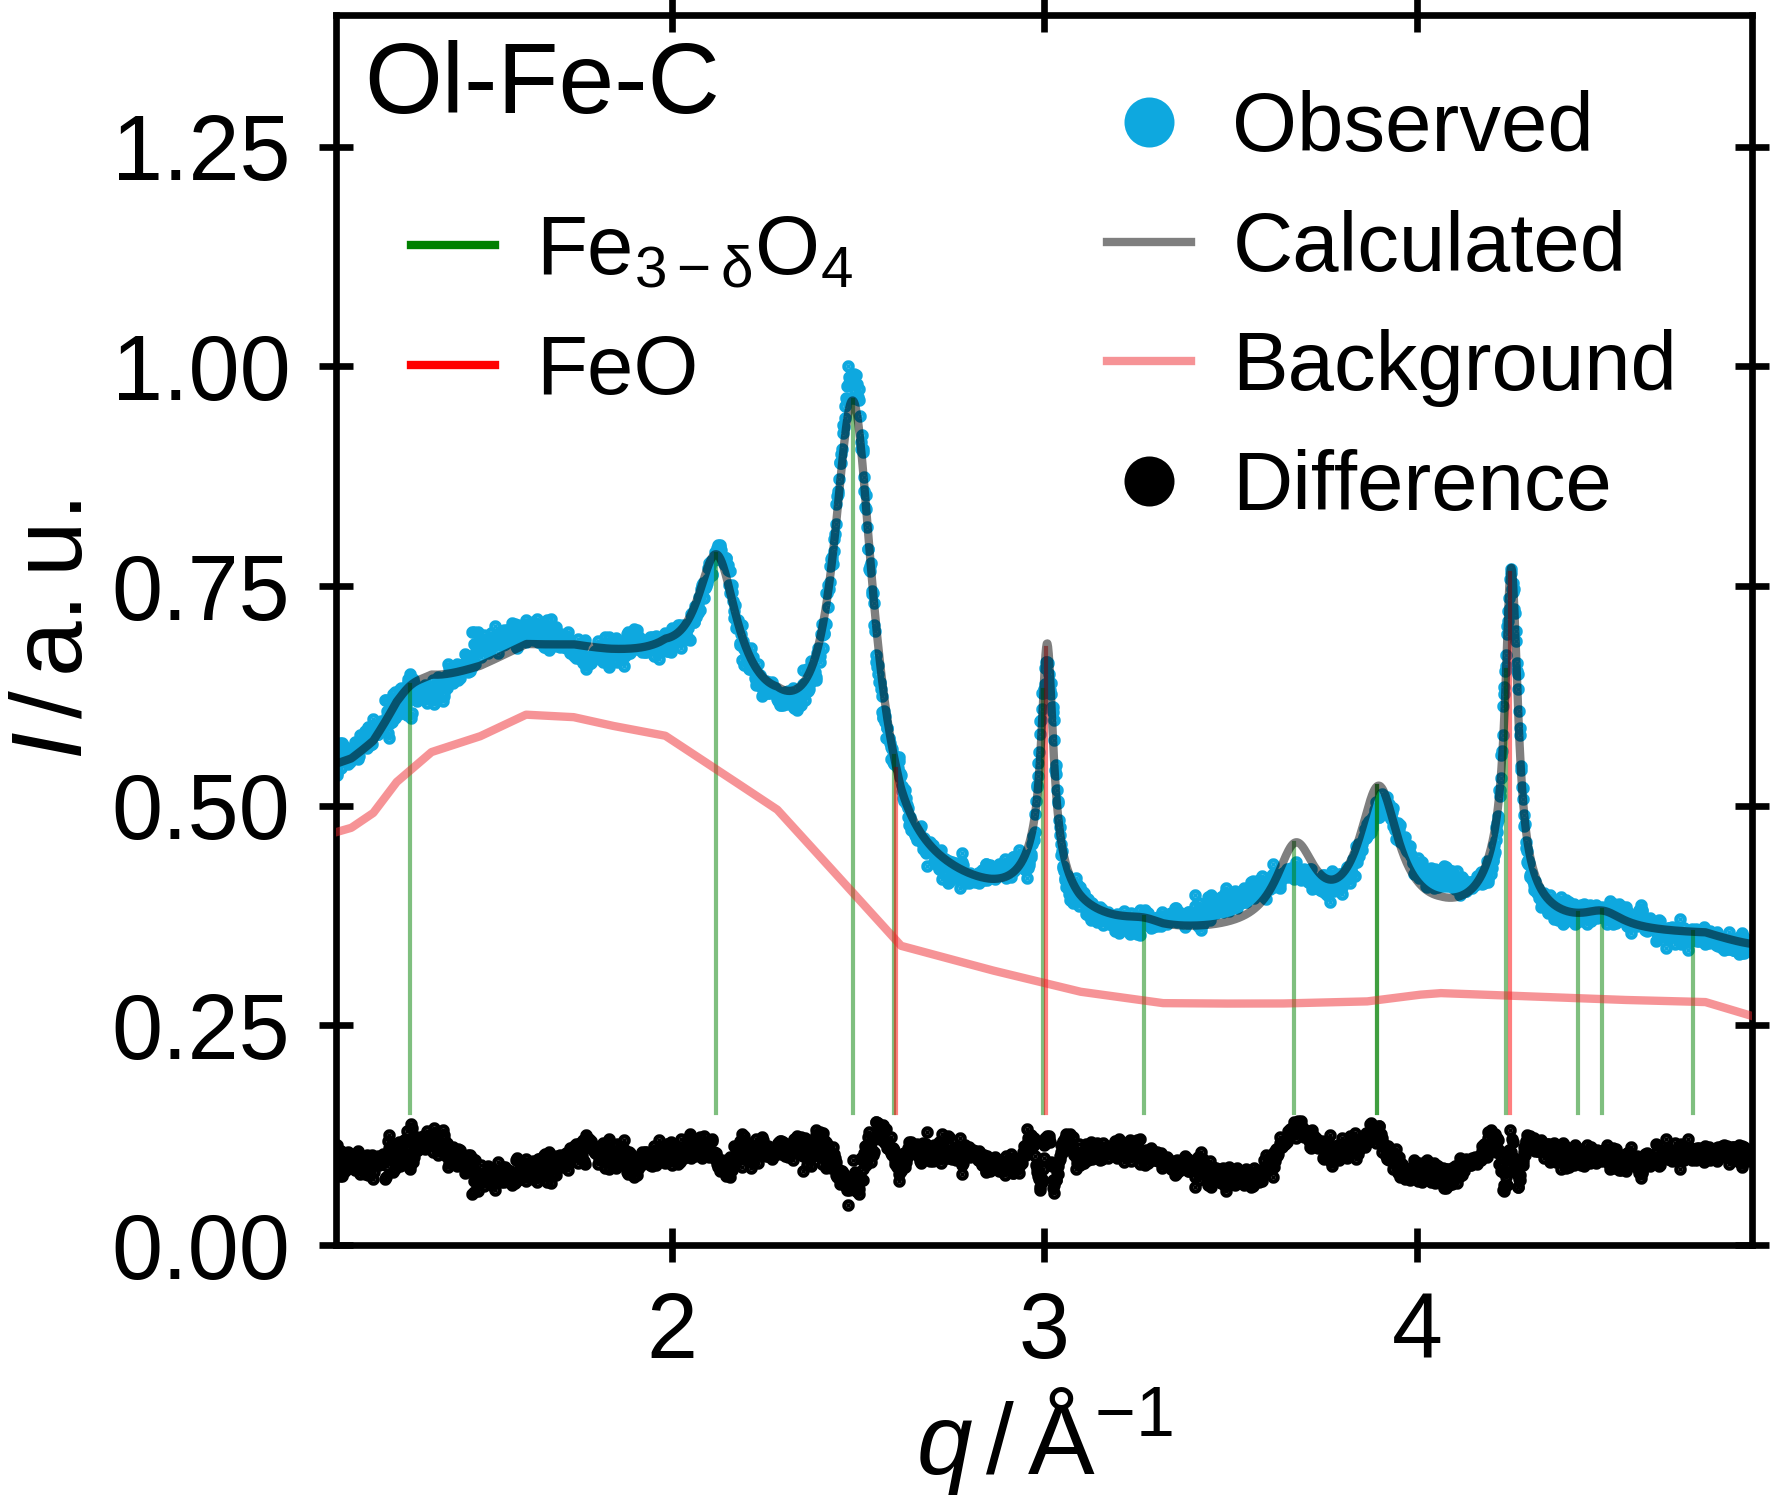
\includegraphics{colloidalCrystals_XRD_Fe3O4WustiteFit_Ol_Fe_C}
    \caption{\label{fig:colloidalCrystals:nanoparticle:xrd}X-ray diffraction of Ol-Fe-C with a LeBail refinement of a combination of an inverse spinell and a w\"ustite phase. The manually estimated background is shown as red line.}
  \end{figure}
  The atomic crystal structure of the nanocubes is studied with X-ray diffraction to confirm the phase composition of the nanoparticles, determine the lattice constants and estimate the crystallite size.
  The XRD in \reffig{fig:colloidalCrystals:nanoparticle:xrd} for Ol-Fe-C shows multiple reflections, which can be associated with an inverse spinell structure.
  The diffractogram is similar to the one measured for iron oxide nanospheres from oleates, which was discussed in \refsec{sec:looselyPackedNS:nanoparticle:xrd}.
  Similarly, two phases are necessary for a proper description, as a closer inspection shows that the reflections around $3 \unit{\angstrom}$ and $4.2 \unit{\angstrom}$ have a lower peak width than the remaining reflections.
  By including a w\"ustite phase, the LeBail refinement yields a close match to the experimental data as shown in \reffig{fig:colloidalCrystals:nanoparticle:xrd}.

  The determined lattice constants $a$ of the two phases, and the Lorentzian isotropic size parameter $Y$ are tabulated together with the determined crystallite sizes $L$ in \reftab{tab:colloidalCrystals:nanoparticle:discussion:xrdLeBail}.

  \begin{table}[ht]
    \centering
    \caption{\label{tab:colloidalCrystals:nanoparticle:discussion:xrdLeBail}Refined parameters of the LeBail fit of Ol-Fe-C. Tabulated are the parameters of the lattice constants $a$, the Lorentzian isotropic size parameter $Y$ and the calculated crystallite size $L$ for both phases. Also given are the used wavelength $\lambda$, the figure of merit $\chi^2$ and the agreement factors $R$.}
    \begin{tabular}{ l | l }
      \hline
      \rule{0pt}{2ex} \textbf{XRD} & \textbf{Ol-Fe-C}\\
      \hline
      \hline
      \rule{0pt}{2ex}space group & $Fd\bar{3}m$ (No. 227) + $Fm\bar{3}m$ (No. 225)\\
      \hline
      \rule{0pt}{2ex} $a_\mathrm{inv. spinell} \,/ \unit{\angstrom}$         &  $8.3841(3)$  \\
      \rule{0pt}{2ex} $Y_\mathrm{inv. spinell} \,/ \unit{^\circ}$            &  $1.776 (6)$   \\
      \rule{0pt}{2ex} $a_\textsf{w\"ustite}     \,/ \unit{\angstrom}$        &  $4.1809(1)$  \\
      \rule{0pt}{2ex} $Y_\textsf{w\"ustite}     \,/ \unit{^\circ}$           &  $0.440(3)$   \\
      \hline
      \rule{0pt}{2ex} $L_\mathrm{inv. spinell} \,/ \unit{nm}$                &  $3.164(2)$ \\
      \rule{0pt}{2ex} $L_\textsf{w\"ustite}      \,/ \unit{nm}$              &  $12.785(4)$ \\
      \hline
      \rule{0pt}{2ex} $\lambda \,/ \unit{\angstrom}$                         &  $1.54056$\\
      \hline
      \rule{0pt}{2ex} $\chi^2$                                               &  $1.70$ \\
      \rule{0pt}{2ex} $R_p \,/ \unit{\%}$                                    &  $1.52$ \\
      \rule{0pt}{2ex} $R_{wp} \,/ \unit{\%}$                                 &  $1.94$ \\
      \rule{0pt}{2ex} $R_{exp} \,/ \unit{\%}$                                &  $1.48$ \\
      \rule{0pt}{2ex} $R_{f, \, \mathrm{inv. spinell}} \,/ \unit{\%}$        &  $0.10$ \\
      \rule{0pt}{2ex} $R_{f, \, \text{w\"ustite}} \,/ \unit{\%}$             &  $0.15$ \\
      \hline
    \end{tabular}
  \end{table}

  The lattice constant of the two phases of Ol-Fe-C as determined by the LeBail fit are $a_\mathrm{inv. spinell} \eq 8.3841(3) \unit{\angstrom}$ for the inverse spinell phase and $a_\textsf{w\"ustite} \eq 4.1809(1) \unit{\angstrom}$ for the w\"ustite phase.
  In comparison to the bulk values of magnetite/maghemite ($a_\mathrm{magnetite} \eq 8.396 \unit{\angstrom}$, $a_\mathrm{maghemite} \eq 8.340 \unit{\angstrom}$) \cite{Cornell_2003_Their} and w\"ustite ($a_\mathrm{FeO} \eq 4.33 \unit{\angstrom}$ \cite{Hentschel_1970_Stoich}), a reduced lattice constant for the w\"ustite phase and a lattice constant close to magnetite for the inverse spinell phase is observed.
  The reduced w\"ustite lattice constant is significantly below the literature value and initial w\"ustite phase values observed in literature for similarly synthesized nanoparticles ($4.265 \unit{\angstrom}$ \cite{Wetterskog_2013_Anoma}).
  On the other hand it is very close to $\tfrac{1}{2} a_\mathrm{inv. spinell}$.
  From literature \cite{Wetterskog_2013_Anoma}, it is known that even after full oxidation of iron oxide nanocubes from oleates, the (400) and (440) reflection of the inverse spinell, at $3 \unit{\angstrom}$ and $4.2 \unit{\angstrom}$ respectively, can have a lower FWHM than the remaining reflections.
  These are the reflections that also overlap with the rock salt structure of w\"ustite.
  The observation of the low w\"ustite lattice constant therefore suggests that not an actual w\"ustite phase is observed in the XRD data, but instead a discrepancy between the long-range order of the tetrahedral and octahedral sublattice in the spinell phase due to anti-phase boundaries that exist throughout the volume of the nanocube from the topotaxial oxidation of the initial w\"ustite phase \cite{Wetterskog_2013_Anoma}.
  It is reasonable to assume that the nanoparticles fully oxidized during the transport to the laboratory in a dry state with direct contact to air.
  The presented LeBail fit that includes a w\"ustite phase is therefore to be understood as a phenomenological description of the data for the anti-phase boundaries.
  % This is analogue to the observations that were made for the iron oxide nanospheres in \refsec{sec:looselyPackedNS:nanoparticle:xrd}.

  With the obtained lattice constants, the mass density of the inverse spinell with an assumed phase of $\ch{Fe3O4}$ is given by $5.22 \unit{g \, mL^{-1}}$ and the assumed w\"ustite phase $\ch{FeO}$ by $6.53 \unit{g \, mL^{-1}}$.
  \\

  The crystallite sizes obtained from the Lorentzian isotropic size parameters $Y$, are $12.785(4) \unit{nm}$ for the w\"ustite core and $3.164(2) \unit{nm}$ for the inverse spinell phase.
  To connect these sizes to the nanocube edge length determined by TEM ($13.42(9) \unit{nm}$), the three-dimensional extensions of the cube have to be considered.
  The space diagonal of the cube from TEM is $\sqrt{3} a \eq 23.2(2) \unit{nm}$ and the space diagonal $\sqrt{2} a \eq 19.0(1) \unit{nm}$.
  The combined crystallite sizes are with $L_\textsf{w\"ustite} + 2 L_\mathrm{inv. spinell} \eq 19.113(6) \unit{nm}$ in between this given range.

  In conclusion, the XRD is phenomenologically described by a two phase system of inverse spinell and w\"ustite.
  A detailed interpretation of the results and comparison with literature information shows however that actually the discrepancy betweeen the octahedral and tetrahedral sublattice in the inverse spinell phase of the iron oxide nanocubes is observed.
  The large size of the w\"ustite crystallites reflects then the topotaxial oxidation of the w\"ustite core to the inverse spinell phase and the small inverse spinell crystallites to the by anti-phase boundaries separated inverse spinell domains.

\end{document}